\chapter{Architecture}\label{ch:arch}

The application is compound by three components:
\begin{enumerate*}[label=(\roman*)]
	\item The scraper, which can be active or not, that uses online
		exchanges API to download market data and save it in a document
		database in a common structure, even if data comes from multiple
		sources;
	\item The server, which accepts requests from the client and runs the
		strategies over the data saved in the database, then it responds
		with the results;
	\item The client, \idest*{the front-end application used by the users to
		submit strategies to the server and get back the results}.
\end{enumerate*}

\begin{figure}[p]
	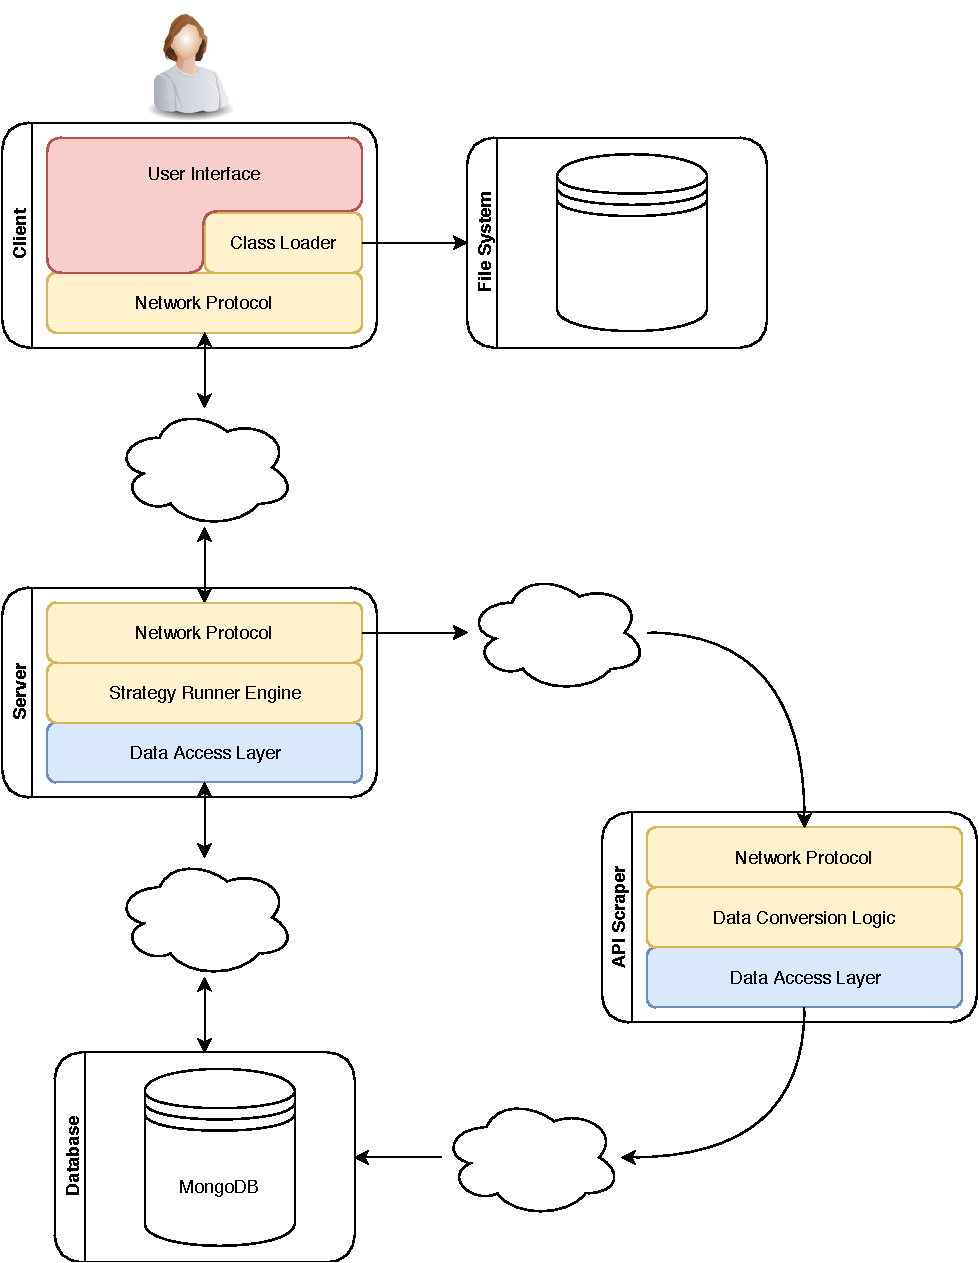
\includegraphics[width=\textwidth]{arch}
	\caption{Application architecture.}
	\label{fig:arch}
\end{figure}

\figref{fig:arch} shows the application's architecture.

\section{Replication and Sharding}\label{sec:distributed}

The application uses replicas to ensure high availability.

All programs that compound the application will always write to the primary
server (as enforced by \mongodb).

The scraper will use the \standout{read preference mode}
\code{primary}, meaning that it will \emph{always} read from the primary server
(if the primary is not online, the read operation will fail). In fact the
scraper needs to be \emph{sure} that the configuration that reads from the
database is the last configuration submitted by the administrator. Moreover,
since the objective of the scraper is to download data and store it in the
database, it would not make sense to run the scraper when the primary server is
not available (the scraper would not be allowed to write to the database).

The server will use the \standout{read preference mode} \code{nearest}, meaning
that it will read from the server with the least network latency. It is in fact
acceptable that some data that the server reads may not be up to date.

To ensure a good load balancing between cluster's servers the \code{Market\-Data}
collection is sharded, because it is the biggest one and it is often read when
running a strategy.

The \code{\_id} field is the shard key since it has a good granularity (so
\mongodb{} can split the documents into a large number of chunks). The field is
hash-indexed, thus the chunks will be randomly distributed across the configured
servers.

\section{Third-party softwares}\label{sec:dependencies}

The following frameworks and libraries are used:
\begin{description}
	\item[Apache Commons CLI v1.4] \textit{(Client, Server)} for parse
		command-line options;
	\item[Gson v2.8.6] \textit{(Scraper)} for JSON deserialization of data
		sources' API responses;
	\item[MongoDB Java Driver v4.0.0] \textit{(Scraper, Server)} for
		handling MongoDB server;
	\item[Retrofit v2.7.2] \textit{(Scraper)} for building HTTP API
		requests;
	\item[XStream v1.4.12] \textit{(All)} for XML
		serialization/deserialization to transmit objects over the
		network.
\end{description}

In the final implementation of the application, newer versions of the
aforementioned dependencies may be used (if they will be released during the
development).

All dependencies are handled with Maven. Other frameworks or libraries may be
added in future.

